
\documentclass[12pt]{article}
\usepackage[a4paper, total={6.5in, 9in}]{geometry}
\usepackage{import}

\import{./}{macros}

\begin{document}
\pagenumbering{roman} % Set page numbering to roman numerals
\fancyhead{} % Clear headers
\renewcommand{\headrulewidth}{0pt} % Remove the header rule

% TITLE PAGE ────────────────────────────────────────────────────────────────────── %
\fancyfoot{} % Hide page number on Title page
% Manual Title Page (For report requirements)
{ % TITLE
    \centering
    % UW Mech/Tron Eng Logo
    
\includegraphics[width=0.75\linewidth]{resources/uwaterloo_mechanical_and_mechatronics_engineering/UWaterloo_Mechanical_Mechatronics_Eng_Logo_vert_rgb.png}
    \sepline
    \centering
    \bf \LARGE
    Final Exam Report\\
    ME 546 - Multi-Sensor Data Fusion
    \sepline
}
\vspace{0.5cm}
{ % AUTHORS
    \centering
    \normalsize\underline{\emph{\quad Prepared by:\quad}}\\
    \vspace{0.5em}
    \large Austin W. Milne \\
    \vspace{1.5em}
    \begin{minipage}[t]{.49\textwidth}
        \centering
        \normalsize\underline{\emph{Course Instructor:}}\\
        \vspace{0.5em}
        \large
        \begin{tabular}{c}
            Prof. Arash Arami \\
        \end{tabular}\\
    \end{minipage}
    \begin{minipage}[t]{.49\textwidth}
        \centering
        \normalsize\underline{\emph{Instructional support:}}\\
        \vspace{0.5em}
        \large
        \begin{tabular}{c}
            Lyndon E. Tang \\
            Mo Shushtari \\
            Eshan Tahvilian \\
        \end{tabular}\\
    \end{minipage}
}
\vfill
\begin{abstract}
    This report was prepared as the Final Exam deliverable for the Winter 2024 offering of ME 546 - Multi-Sensor Data Fusion at the University of Waterloo. The report covers the design, implementation, and results of three problems: Multi Tracking Kalman Filter, Ball Tracking with Bayesian Fusion, and Neural Network Estimation of Walking Gate Ground Force.
\end{abstract}
{ % DATE
    \centering
    \large
    April 19th, 2024\\ 
}
\clearpage
\fancyfoot[C]{\thepage} % Enable page numbers again

% TABLE OF CONTENTS AND OTHER TABLES ────────────────────────────────────────────── %
\clearpage
\tableofcontents
\clearpage

\listoftables % Comment out if no tables.
\listoffigures % Comment out if no figures.
\listofequations % Commend out if no equations.
% \lstlistoflistings % Comment out if there are no listings.

% MOTIVATION ────────────────────────────────────────────────────────────────────── %
\clearpage
\pagenumbering{arabic} % Reset page number to arabic numbers, restart numbering.
\section{Problem 1 - Multi Tracking Extended Kalman Filter}
Problem 1 focuses on creating a multi-fish tracking filter for a sonar based fish detector. The sensor provides range, angle, and size measurements for each fish during a measurement sweep of the sonar. The goal is to track the position and size of each fish that appears in the sonar range. An extended Kalman Filter is used to estimate the position and size of each fish.

\begin{figure}[H]
    \centering
    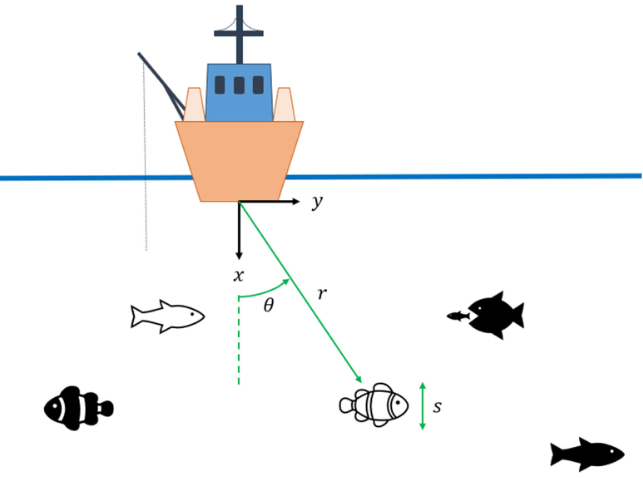
\includegraphics[width=0.99\textwidth]{Problem 1/assets/Sensor-Context.png}
    \caption{Sonar fish tracking system \cite{final-exam}}
    \label{fig:p1-sonar}
\end{figure}

The sensor suffers from measurement noise, which is characterized by the variance of the range, angle, and size measurements. The sensor can also briefly lose "sight" of a fish and then reacquire it. The process noise is unknown, but the filter is tuned to provide the most accurate tracking results.

For this system an Extended Kalman Filter is necessary since the relation between the state and the measurements is nonlinear. Since the noise of each sensor is relative to its own axis, a coordinate transfer needs to happen within the statistical calculations. The EKF facilitates this by providing a linear approximation and a Jacobian matrix for the sensor models.

\subsection{Extended Kalman Filter Design}
The EKF is designed to track the position and size of each fish. In order to better predict the movement, the velocity and acceleration of each fish are also tracked. The result is a 7-state EKF Filter that tracks the position, velocity, and acceleration in the X and Y axis along with the size of the fish:

\begin{equation}
    \label{eqn:p1-state-vector}
    x = \begin{bmatrix}
        x \\ y \\ \dot{x} \\ \dot{y} \\ \ddot{x} \\ \ddot{y} \\ s
    \end{bmatrix}
\end{equation}
\equations{State vector for the Kalman Filter}

With the understanding that the differential equation for the process model ($F$) can be described as:
\begin{equation}
    \label{eqn:p1-diff-eqn}
    x = F x
\end{equation}

\begin{equation}
    \label{eqn:p1-process-model}
    F = \frac{\partial f(x)}{\partial x} = \begin{bmatrix}
        1 & 0 & \Delta t & 0 & \frac{1}{2} \Delta t^2 & 0 & 0 \\
        0 & 1 & 0 & \Delta t & 0 & \frac{1}{2} \Delta t^2 & 0 \\
        0 & 0 & 1 & 0 & \Delta t & 0 & 0 \\
        0 & 0 & 0 & 1 & 0 & \Delta t & 0 \\
        0 & 0 & 0 & 0 & 1 & 0 & 0 \\
        0 & 0 & 0 & 0 & 0 & 1 & 0 \\
        0 & 0 & 0 & 0 & 0 & 0 & 1 \\
    \end{bmatrix}
\end{equation}
\equations{Process model for the Kalman Filter}

\subsubsection{Sensor Models}

Each of the sensor conversion functions are very simple, just converting the range and angle measurements into Cartesian coordinates. The Jacobian is also computed for each sensor relative to the state vector. The models are shown below. Range sensor:

\begin{equation}
    \label{eqn:p1-range-model}
    \begin{gathered}
        h_{r} = r = \sqrt{x^2 + y^2} \\
        H_{r} = \left. \frac{\partial h_{r}}{\partial x} \right|_x =
        \begin{bmatrix}
            \frac{x}{\sqrt{x^2 + y^2}} \\ \frac{y}{\sqrt{x^2 + y^2}} \\ 0 \\ 0 \\ 0 \\ 0 \\ 0
        \end{bmatrix}
    \end{gathered}
\end{equation}
\equations{Range sensor model for the Kalman Filter}

Angle sensor:

\begin{equation}
    \label{eqn:p1-angle-model}
    \begin{gathered}
        h_{\theta} = \theta = \tan^{-1} \left( \frac{y}{x} \right) \\
        H_{\theta} = \left. \frac{\partial h_{\theta}}{\partial x} \right|_x =
        \begin{bmatrix}
            -\frac{y}{x^2 + y^2} \\ \frac{x}{x^2 + y^2} \\ 0 \\ 0 \\ 0 \\ 0 \\ 0
        \end{bmatrix}
    \end{gathered}
\end{equation}
\equations{Angle sensor model for the Kalman Filter}

Finally, the size sensor:

\begin{equation}
    \label{eqn:p1-size-model}
    \begin{gathered}
        h_{s} = s \\
        H_{s} = \left. \frac{\partial h_{s}}{\partial x} \right|_x =
        \begin{bmatrix}
            0 \\ 0 \\ 0 \\ 0 \\ 0 \\ 0 \\ 1
        \end{bmatrix}
    \end{gathered}
\end{equation}
\equations{Size sensor model for the Kalman Filter}

\subsubsection{Covariance Matrices}\label{sec:p1-covariance-matrices}
The process noise covariance matrix ($Q$) and the measurement noise covariance matrix ($R$) are crucial to creating a well-tuned Kalman Filter, allowing it to accurately determine the statistical properties of the noise in the system. The measurement noise could be directly calculated from the training data. Figures \ref{fig:p1-sorted-size-hist} and \ref{fig:p1-sorted-pos-plot} show the radar sensor readings grouped with their respective fish. For readability, the position is shown in Cartesian coordinates.

% Size Reading Graphs
\begin{figure}[H]
    \centering
    \begin{subfigure}[b]{0.49\textwidth}
        \centering
        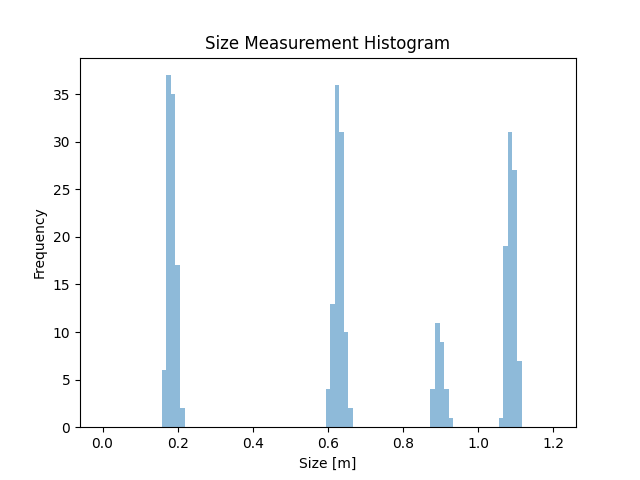
\includegraphics[width=\textwidth]{Problem 1/out/p1_size_hist.png}
        \caption{Reading histogram}
        \label{fig:p1-size-hist}
    \end{subfigure}
    \begin{subfigure}[b]{0.49\textwidth}
        \centering
        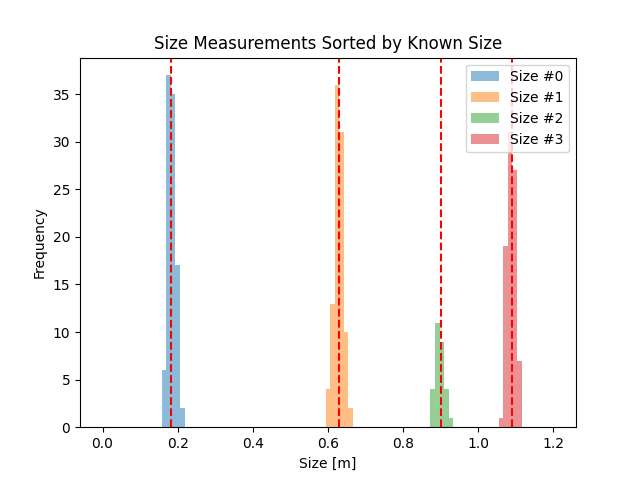
\includegraphics[width=\textwidth]{Problem 1/out/p1_sorted_size_hist.png}
        \caption{Grouped reading histogram}
        \label{fig:p1-sorted-size-hist}
    \end{subfigure}
    \caption{Training data size measurements}
    \label{fig:p1-size-hists}
\end{figure}

% Position Reading Graphs
\begin{figure}[H]
    \centering
    \begin{subfigure}[b]{0.49\textwidth}
        \centering
        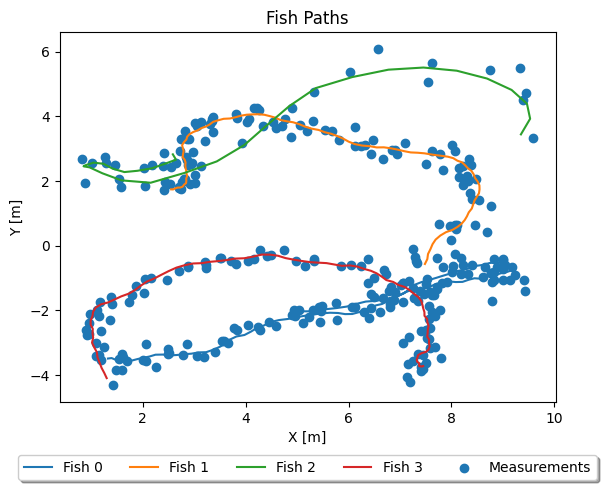
\includegraphics[width=\textwidth]{Problem 1/out/p1_pos_plot.png}
        \caption{Unsorted plot}
        \label{fig:p1-pos-plot}
    \end{subfigure}
    \begin{subfigure}[b]{0.49\textwidth}
        \centering
        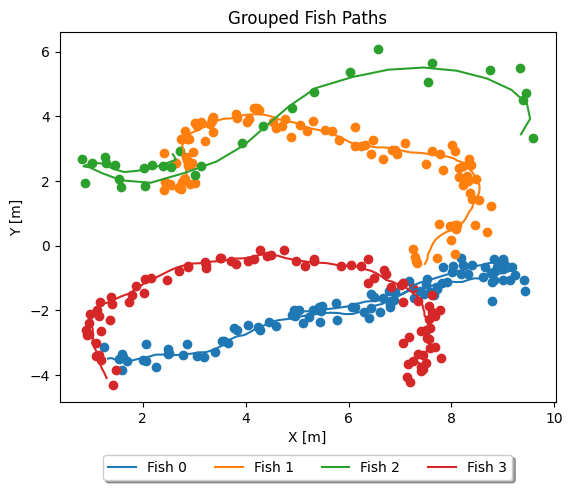
\includegraphics[width=\textwidth]{Problem 1/out/p1_sorted_pos_plot.png}
        \caption{Sorted plot}
        \label{fig:p1-sorted-pos-plot}
    \end{subfigure}
    \caption{Training data position measurements in Cartesian coordinates}
    \label{fig:p1-pos-plots}
\end{figure}

Figures \ref{fig:p1-size-error} and \ref{fig:p1-pos-error} then show the error distributions for the size and position measurements. The error is determined to be the distance in the relevant measurement from readout to actual. The variance of the measurements is then calculated and shown in Table \ref{tab:p1-meas-noise}.

% Size Error Distribution
\begin{figure}[H]
    \centering
    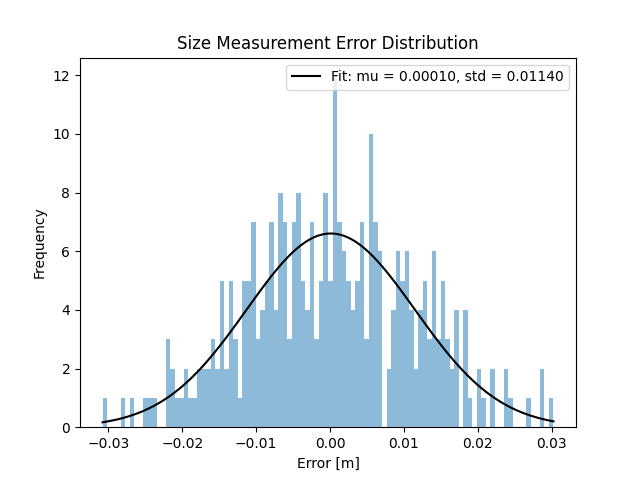
\includegraphics[width=0.75\textwidth]{Problem 1/out/p1_size_error_hist.png}
    \caption{Training data size reading error distribution}
    \label{fig:p1-size-error}
\end{figure}

% Position Error Distributions
\begin{figure}[H]
    \centering
    \begin{subfigure}[b]{0.49\textwidth}
        \centering
        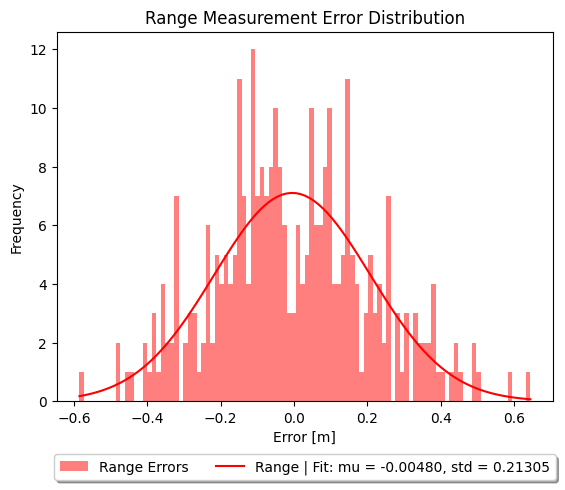
\includegraphics[width=\textwidth]{Problem 1/out/p1_r_pos_error_hist.png}
        \caption{Range error distribution}
        \label{fig:p1-r-pos-error}
    \end{subfigure}
    \begin{subfigure}[b]{0.49\textwidth}
        \centering
        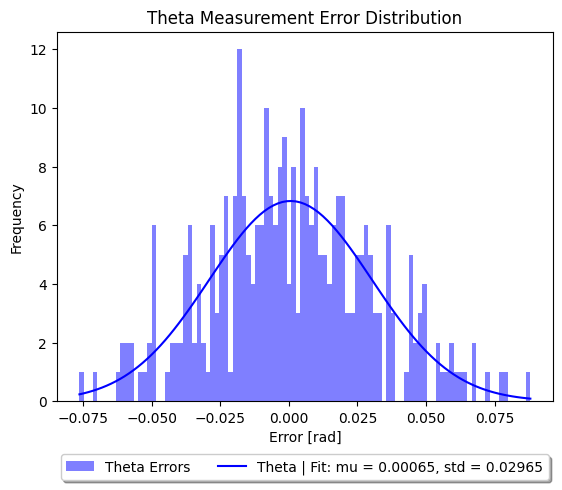
\includegraphics[width=\textwidth]{Problem 1/out/p1_t_pos_error_hist.png}
        \caption{$\theta$ error distribution}
        \label{fig:p1-t-pos-error}
    \end{subfigure}
    \caption{Training data position measurement error distributions}
    \label{fig:p1-pos-error}
\end{figure}

\begin{table}[H]
    \centering
    \caption{Measurement variances}
    \label{tab:p1-meas-noise}
    \begin{tabular}{|c|c|}
        \hline
        \textbf{Measurement} & \textbf{Variance} ($\sigma^2$) \\
        \hline
        Range &    0.04539078586229167 \\
        \hline
        $\theta$ & 0.00087889950813572 \\
        \hline
        Size &     0.00012988333066048 \\
        \hline
    \end{tabular}
\end{table}

The measurement noise covariance matrix is then decided to be the diagonal matrix of the variances of the measurements:

\begin{equation}
    \label{eqn:p1-meas-noise-cov}
    R = \begin{bmatrix}
        0.0453\dots & 0 & 0 \\
        0 & 0.0008\dots & 0 \\
        0 & 0 & 0.0001\dots
    \end{bmatrix}
\end{equation}
\equations{Measurement noise covariance matrix}

The process noise covariance matrix is more complicated to determine. As an alternative to the traditional approach of trying to profile the process noise from analysis of the reference truth data, the process noise is instead tuned to provide the best tracking results.

The process noise matrix is determined to be a diagonal matrix with the following values:

\begin{equation}
    \label{eqn:p1-proc-noise-cov}
    Q = \begin{bmatrix}
        \sigma^2_{x,y} & 0 & 0 & 0 & 0 & 0 & 0 \\
        0 & \sigma^2_{x,y} & 0 & 0 & 0 & 0 & 0 \\
        0 & 0 & \sigma^2_{\dot{x},\dot{y}} & 0 & 0 & 0 & 0 \\
        0 & 0 & 0 & \sigma^2_{\dot{x},\dot{y}} & 0 & 0 & 0 \\
        0 & 0 & 0 & 0 & \sigma^2_{\ddot{x},\ddot{y}} & 0 & 0 \\
        0 & 0 & 0 & 0 & 0 & \sigma^2_{\ddot{x},\ddot{y}} & 0 \\
        0 & 0 & 0 & 0 & 0 & 0 & \sigma^2_{s}
    \end{bmatrix}
\end{equation}

The model with the Q matrix was run against the training data and the average root mean squared error (RMSE) was calculated. The $\sigma^2_{x,y}$, $\sigma^2_{\dot{x},\dot{y}}$, $\sigma^2_{\ddot{x},\ddot{y}}$, and $\sigma^2_{s}$ values were then tuned using a differential evolution optimization algorithm \cite{scipy} to minimize the RMSE. This was done for the entire known path of fishes 0 and 1 in the training data. The final values where averaged from fishes 0 and 1 and the resulting values are shown in Table \ref{tab:p1-tuned-proc-noise}.

\begin{table}[H]
    \centering
    \caption{Tuned process noise variances}
    \label{tab:p1-tuned-proc-noise}
    \begin{tabular}{|c|c|}
        \hline
        \textbf{Process Noise} & \textbf{Variance} ($\sigma^2$) \\
        \hline
        $\sigma^2_{x,y}$ & $0.0011501322599521454$ \\
        \hline
        $\sigma^2_{\dot{x},\dot{y}}$ & $0.06870244206669615$ \\
        \hline
        $\sigma^2_{\ddot{x},\ddot{y}}$ & $0.0$ \\
        \hline
        $\sigma^2_{s}$ & $1.5510976521855614 \times 10^{-07}$ \\
        \hline
    \end{tabular}
\end{table}

The resultant process noise covariance matrix is then:

\begin{equation}
    \label{eqn:p1-tuned-proc-noise-cov}
    Q = \begin{bmatrix}
        0.00115\dots & 0 & 0 & 0 & 0 & 0 & 0 \\
        0 & 0.00115\dots & 0 & 0 & 0 & 0 & 0 \\
        0 & 0 & 0.06870\dots & 0 & 0 & 0 & 0 \\
        0 & 0 & 0 & 0.06870\dots & 0 & 0 & 0 \\
        0 & 0 & 0 & 0 & 0 & 0 & 0 \\
        0 & 0 & 0 & 0 & 0 & 0 & 0 \\
        0 & 0 & 0 & 0 & 0 & 0 & 1.55109\dots \times 10^{-07}
    \end{bmatrix}
\end{equation}
\equations{Process noise covariance matrix}

To ensure that the process noise covariance matrix is reasonable, the filter was run against the training data of fish 0. The resultant path, size, and z-score calculation (important for section \ref{sec:p1-multi-fish-tracking}) are shown in figure \ref{fig:p1-test-fish-0}. The plot shows reasonably accurate tracking of the fish.

\begin{figure}[H]
    \centering
    \begin{subfigure}[b]{0.49\textwidth}
        \centering
        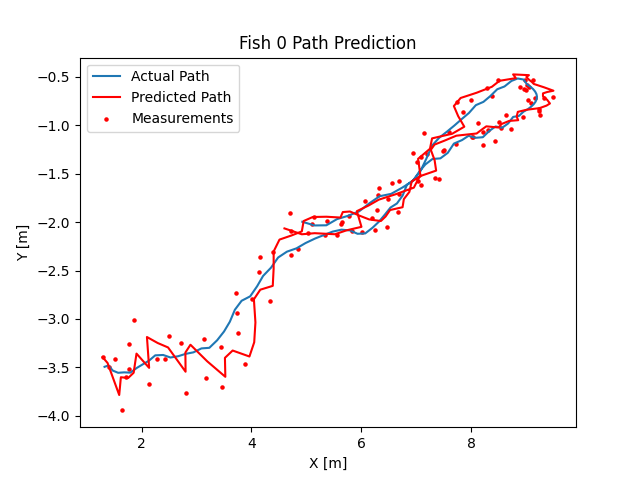
\includegraphics[width=\textwidth]{Problem 1/out/p1_test_fish_0_path.png}
        \caption{Path Prediction}
        \label{fig:p1-test-fish-0-path}
    \end{subfigure}
    \begin{subfigure}[b]{0.49\textwidth}
        \centering
        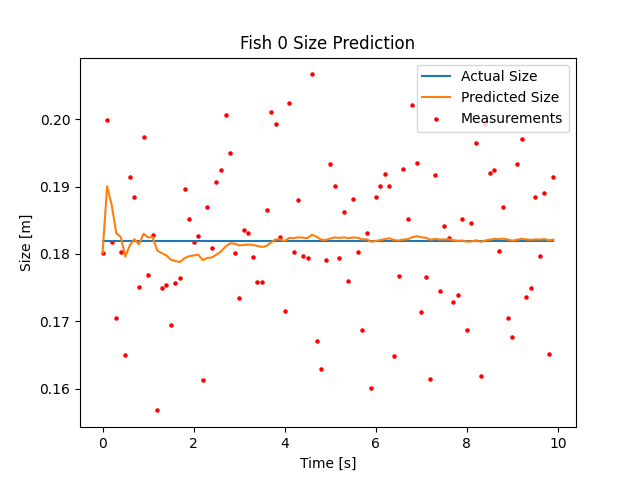
\includegraphics[width=\textwidth]{Problem 1/out/p1_test_fish_0_size.png}
        \caption{Error Prediction}
        \label{fig:p1-test-fish-0-size}
    \end{subfigure}
    \begin{subfigure}[b]{0.49\textwidth}
        \centering
        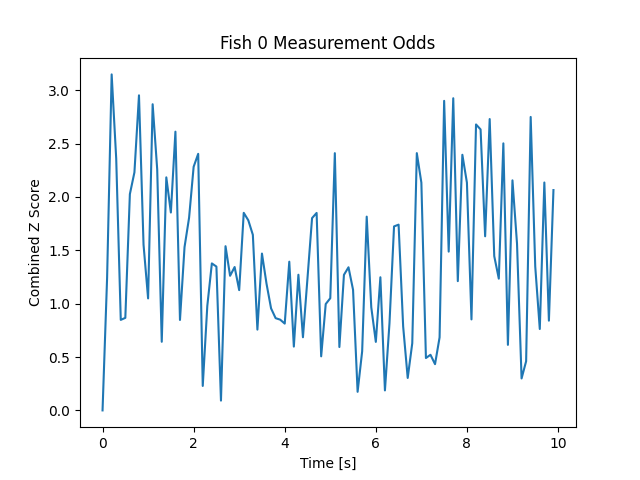
\includegraphics[width=\textwidth]{Problem 1/out/p1_test_fish_0_odds.png}
        \caption{Path Prediction}
        \label{fig:p1-test-fish-0-odds}
    \end{subfigure}
    \caption{Test fish 0 prediction}
    \label{fig:p1-test-fish-0}
\end{figure}

\subsection{Extended Kalman Filter Implementation}
The extended kalman filter (EKF) was implemented using an existing EKF class from the FilterPy library \cite{filterpy}. The EKF class provides the basic update a predict functions for the filter as well as storage for the current state and covariance matrices. The EKF class was wrapped in a custom EKF class to handle other useful functions. The most useful functions implemented are the \lstinline{z_score_of_measurement_match}, \lstinline{score_pos_accuracy}, and \lstinline{score_size_accuracy} functions. The \lstinline{z_score_of_measurement_match} function calculates the z-score of a given measurement as the next value of the filter's series. This is the sum of the X and Y axis z-scores. This is used in section \ref{sec:p1-multi-fish-tracking} for assigning measurements to tracks. The \lstinline{score_pos_accuracy} and \lstinline{score_size_accuracy} functions calculate the accuracy of the position and size predictions from a set of data inputs. These are used in section \ref{sec:p1-covariance-matrices} to optimize the process noise covariance matrix. The source code for the EKF is included in \ref{appendix-p1-code} and in the additional resources of this report submission.

\subsection{Multi Fish Tracking}\label{sec:p1-multi-fish-tracking}
The multi-fish tracking algorithm is implemented by running the EKF on each fish in the sonar sweep. Due to the errors and irregularities in the data as outlined above, some logical operations are needed to assign sensor readings to the correct fish's EKF. The algorithm is as follows:

\begin{enumerate}
    \item For every combination of existing fish and new measurements:
    \begin{enumerate}
        \item Predict the next EKF size
        \item Calculate the z-score of the size measurement match
        \item if the size z-score is above a threshold: Store a position z-score of inifinity
        \item else:
        \begin{enumerate}
            \item Predict the next EKF position
            \item Calculate the z-score of the position measurement match
            \item Store the position z-score
        \end{enumerate}
    \end{enumerate}
    \item Until there are no position z-score left below the threshold
    \begin{enumerate}
        \item Find the lowest z-score
        \item Update the relevant fish with the relevant measurement
    \end{enumerate}
    \item For every measurement that has not been assigned to a fish:
    \begin{enumerate}
        \item Create a fish tracker EKF
        \item Initialize the EKF with the measurement
    \end{enumerate}
    \item For every fish that has not been assigned a measurement:
    \begin{enumerate}
        \item Predict the next EKF position
        \item Increment the fish's count of missed measurements
    \end{enumerate}
    \item If a fish has missed too many measurements:
    \begin{enumerate}
        \item Remove the tracker
        \item Remove positions after loss of signal from position history
    \end{enumerate}
\end{enumerate}

This combination of logic allows the filter to accurately track multiple fish in the sonar sweep while overlooking missed measurements and allowing for fish to appear and disappear independently.

Manual tuning of the parameters such as z-score limits and missed measurement limits was necessary to ensure the filter was tracking accurately. The final parameters are available in the source code in \ref{appendix-p1-code}. The final results of running the multitracking filter on the training data are shown in figure \ref{fig:p1-training-prediction}.

\begin{figure}[H]
    \centering
    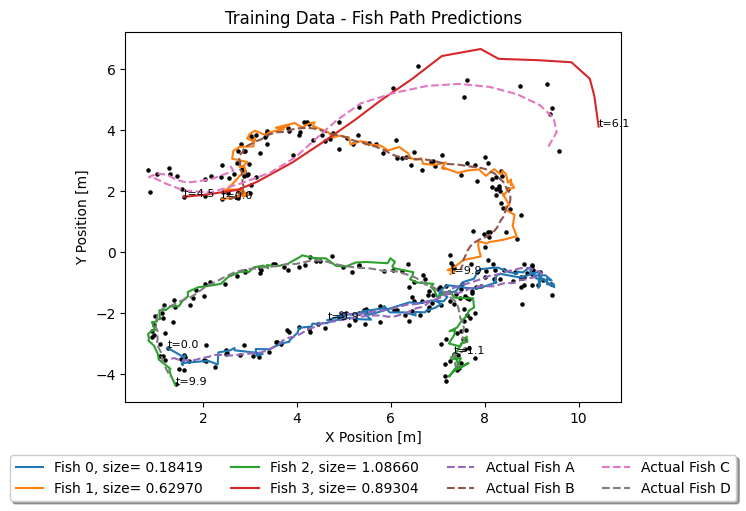
\includegraphics[width=0.99\textwidth]{Problem 1/out/p1_training_paths.png}
    \caption{Training data multi fish tracking prediction compared to real paths}
    \label{fig:p1-training-prediction}
\end{figure}

The tracking is satisfactorily accurate, with the fish paths closely matching the real paths. Predicted fish 3, corresponding to actual fish C, is not tracked as accurately as the other fish. This is likely due to the more rapid movement and higher acceleration compared to the other fish. Fish 3-C moves faster than fish 0 and fish 1 that were used for the process noise tuning in section \ref{sec:p1-covariance-matrices}. This would lead to the filter being more sluggish to update the acceleration component of the state vector. The result is the overshoot in the region of $(7 < x < 11, 4 < y < 7)$. Performance could likely be improved by manually tuning the process past the existing state, specifically in these types of edge cases.

\subsection{Fish Tracking Results}
Finally, the filter was applied to the test data. The results are shown in figure \ref{fig:p1-test-prediction}. The final positions and sizes of the fish are shown in table \ref{tab:p1-test-results}. The final covariance matrices for each fish are shown in table \ref{tab:p1-test-cov}. While the position tracks are not smooth, they do a decent job of following the fishs' paths. The size predictions are expected to be very accurate, as they proved to be with tests in the training data.

\begin{figure}[H]
    \centering
    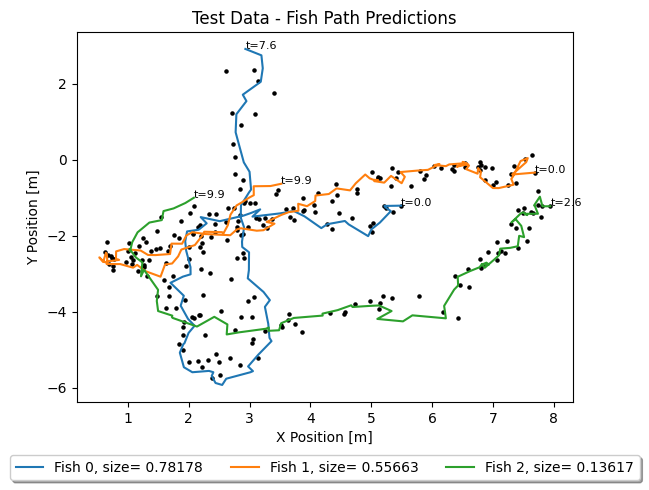
\includegraphics[width=0.99\textwidth]{Problem 1/out/p1_test_paths.png}
    \caption{Test data multi fish tracking prediction}
    \label{fig:p1-test-prediction}
\end{figure}

\begin{table}[H]
    \centering
    \caption{Fish tracking results}
    \label{tab:p1-test-results}
    \begin{tabular}{|c|c|c|c|c|c|}
        \hline
        \textbf{Fish \#} & \textbf{Size} & \textbf{Time Start} & \textbf{Time End} & \textbf{Final X [m]} & \textbf{Final Y [m]}\\
        \hline
        Fish 0 & +0.7813 & +0.0000 & +7.6000 & +2.9447 & +2.9158\\
        Fish 1 & +0.5564 & +0.0000 & +9.9000 & +3.5141 & -0.6288\\
        Fish 2 & +0.1361 & +2.6000 & +9.9000 & +2.1045 & -1.0043\\
        \hline
    \end{tabular}
\end{table}

The covariance matrices (table \ref{tab:p1-test-cov}) show that the filter is confident in the position and size of the fish. The position variance being in the range of $0.015$ to $0.031$ and the size variance being less than $0.001$ for all fish. For comparison, figure \ref{fig:p1-pos-error-hist} shows the error distribution of the raw position measurements if converted to Cartesian coordinates. The raw measurements provide a position variance of around $0.068$, meaning that the filter has about have the uncertainty of the raw measurements, in addition to multitarget tracking functionality.

\begin{table}[H]
    \centering
    \caption{Fish tracking covariance matrices}
    \label{tab:p1-test-cov}
    \begin{tabular}{|c|c|}
        \hline
        \textbf{Fish \#} & \textbf{Final Covariance Matrix}\\
        \hline
        Fish 0 & $\begin{bmatrix}
            +0.026 & +0.007 & +0.049 & +0.010 & +0.007 & +0.001 & +0.000 \\
            +0.007 & +0.023 & +0.009 & +0.045 & +0.001 & +0.006 & +0.000 \\
            +0.049 & +0.009 & +0.259 & +0.016 & +0.034 & +0.002 & +0.000 \\
            +0.010 & +0.045 & +0.016 & +0.248 & +0.002 & +0.033 & +0.000 \\
            +0.007 & +0.001 & +0.034 & +0.002 & +0.052 & +0.000 & +0.000 \\
            +0.001 & +0.006 & +0.002 & +0.033 & +0.000 & +0.052 & +0.000 \\
            +0.000 & +0.000 & +0.000 & +0.000 & +0.000 & +0.000 & +0.000 \\
        \end{bmatrix}$\\
        \hline
        Fish 1 & $\begin{bmatrix}
            +0.031 & -0.004 & +0.055 & -0.005 & +0.006 & -0.000 & +0.000 \\
            -0.004 & +0.015 & -0.005 & +0.033 & -0.001 & +0.003 & +0.000 \\
            +0.055 & -0.005 & +0.264 & -0.010 & +0.027 & -0.001 & +0.000 \\
            -0.005 & +0.033 & -0.010 & +0.225 & -0.001 & +0.023 & +0.000 \\
            +0.006 & -0.001 & +0.027 & -0.001 & +0.039 & -0.000 & +0.000 \\
            -0.000 & +0.003 & -0.001 & +0.023 & -0.000 & +0.039 & +0.000 \\
            +0.000 & +0.000 & +0.000 & +0.000 & +0.000 & +0.000 & +0.000 \\
        \end{bmatrix}$\\
        \hline
        Fish 2 & $\begin{bmatrix}
            +0.026 & -0.009 & +0.049 & -0.013 & +0.007 & -0.002 & +0.000 \\
            -0.009 & +0.016 & -0.015 & +0.033 & -0.002 & +0.005 & +0.000 \\
            +0.049 & -0.015 & +0.255 & -0.026 & +0.035 & -0.004 & +0.000 \\
            -0.013 & +0.033 & -0.026 & +0.231 & -0.004 & +0.032 & +0.000 \\
            +0.007 & -0.002 & +0.035 & -0.004 & +0.055 & -0.000 & +0.000 \\
            -0.002 & +0.005 & -0.004 & +0.032 & -0.000 & +0.054 & +0.000 \\
            +0.000 & +0.000 & +0.000 & +0.000 & +0.000 & +0.000 & +0.000 \\
        \end{bmatrix}$\\
        \hline
    \end{tabular}
\end{table}

\begin{figure}[H]
    \centering
    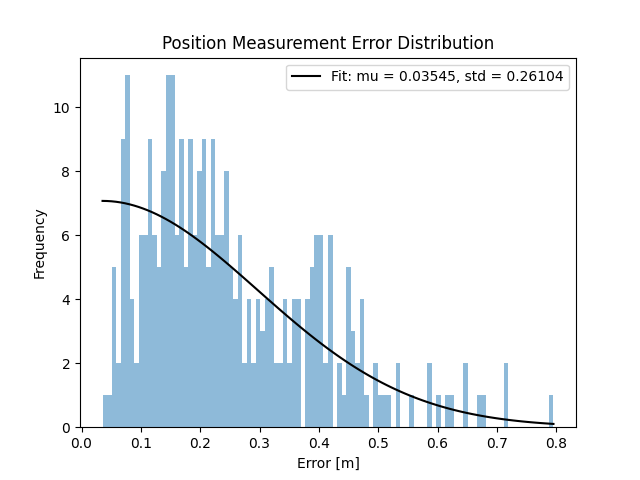
\includegraphics[width=0.99\textwidth]{Problem 1/out/p1_pos_error_hist.png}
    \caption{Training data cartesian position error distribution}
    \label{fig:p1-pos-error-hist}
\end{figure}

As requested in final exam document \cite{final-exam}, a CSV file is provided that contains the count of number of tracked fish at each time step. The count of fish over time is also shown in figure \ref{fig:p1-fish-count}.

\begin{figure}[H]
    \centering
    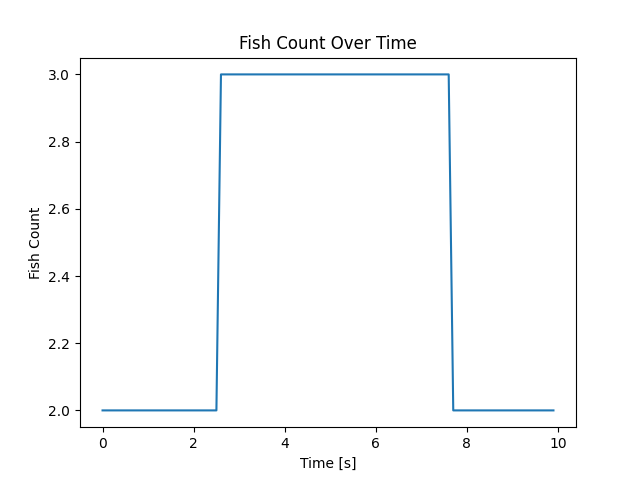
\includegraphics[width=0.99\textwidth]{Problem 1/out/p1_fish_count.png}
    \caption{Fish count over time}
    \label{fig:p1-fish-count}
\end{figure}

\section{Problem 2 - Ball Tracking with Bayesian Fusion}
Problem 2 focuses on using a Bayesian filter to predict the shot placement of a ball after it has been kicked at specific contact patch or a mixture of contact patches. Figure \ref{fig:p2-reference-frame} shows the reference frame for the ball and the relevant contact patches.

\begin{figure}[H]
    \centering
    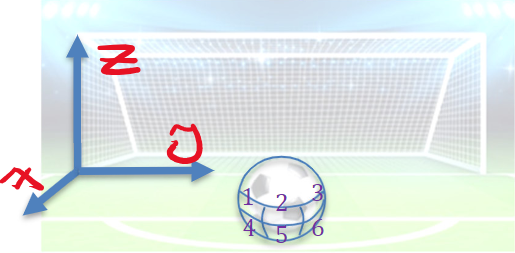
\includegraphics[width=0.99\textwidth]{Problem 2/assets/axis-plane.png}
    \caption{Reference frame for ball contact and tracking \cite{final-exam}}
    \label{fig:p2-reference-frame}
\end{figure}

Figure \ref{fig:p2-kicks-by-contact-area} shows the scatter plot of kick data provided. As is to be expected, the data is varied, but shows a trend of placement being in the opposite Y and Z direction from the contact patch. The data is labelled by color for each contact patch.

\begin{figure}[H]
    \centering
    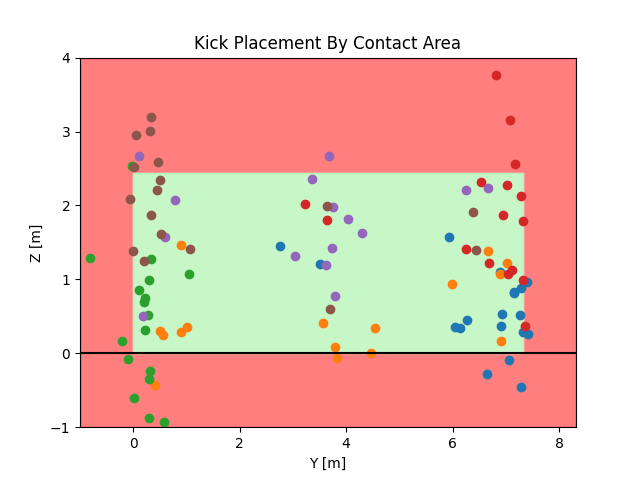
\includegraphics[width=0.99\textwidth]{Problem 2/out/kick_plot_by_contact_area.png}
    \caption{Kick placement scatter organized by contact area}
    \label{fig:p2-kicks-by-contact-area}
\end{figure}

\subsection{Contact Area Probability}
With the data provided, a probability field was created for a kick placed at each contact patch. Figure \ref{fig:p2-distributions} shows the individual distributions for each contact patch, while figure \ref{fig:p2-normalized-distributions} shows the normalized distributions. From the figured, it is evident that kicks from contact patch 3 are the most consistent, with contact patch 1 being the next most consistent and contact patch 2 having the most varied results. Table \ref{tab:p2-distribution-stats} shows the mean and variance of the distributions for each contact patch.

\begin{figure}[H]
    \begin{subfigure}[b]{0.99\textwidth}
        \centering
        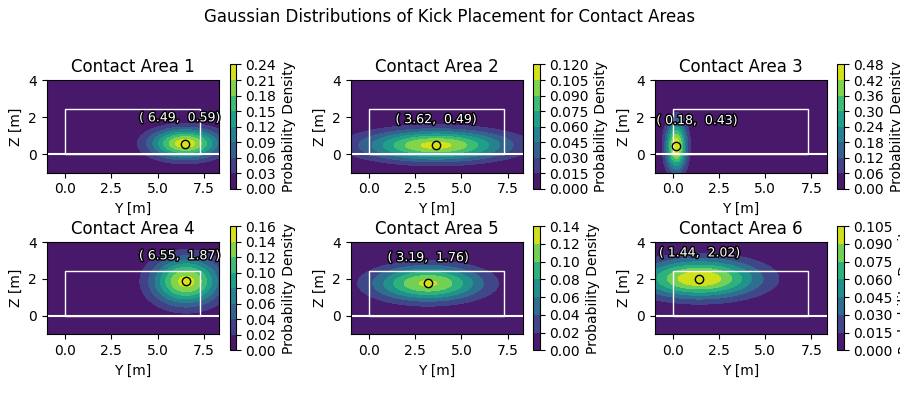
\includegraphics[width=\textwidth]{Problem 2/out/contact_area_probability_dist.png}
        \caption{Individual distributions}
        \label{fig:p2-distributions}
    \end{subfigure}
    \begin{subfigure}[b]{0.99\textwidth}
        \centering
        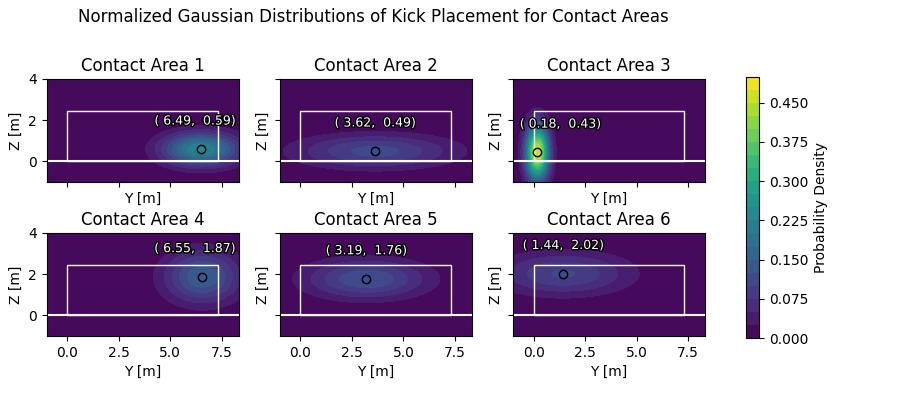
\includegraphics[width=\textwidth]{Problem 2/out/normalized_contact_area_probability_dist.png}
        \caption{Normalized distributions}
        \label{fig:p2-normalized-distributions}
    \end{subfigure}
    \caption{Kick result probability distributions by contact area}
    \label{fig:p2-both-distributions}
\end{figure}

\begin{table}[H]
    \centering
    \caption{Contact area probability statistics}
    \label{tab:p2-distribution-stats}
    \begin{tabular}{|c|c|c|c|c|}
        \hline
        \textbf{Contact Area} & \textbf{Y Mean} [m] & \textbf{Y Variance} & \textbf{Z Mean} [m] & \textbf{Z Variance}\\
        \hline
        1 & 6.4937 & 1.6403 & 0.5852 & 0.2991\\
        \hline
        2 & 3.6229 & 6.7131 & 0.4883 & 0.3116\\
        \hline
        3 & 0.1790 & 0.1422 & 0.4347 & 0.8120\\
        \hline
        4 & 6.5535 & 1.5737 & 1.8657 & 0.7385\\
        \hline
        5 & 3.1949 & 3.9846 & 1.7620 & 0.4180\\
        \hline
        6 & 1.4352 & 4.7952 & 2.0183 & 0.4953\\
        \hline
    \end{tabular}
\end{table}

\subsection{Bayesian Fusion}
Since each contact patch has its own probability field, the Bayesian fusion can be used to combine the information from each contact patch with the influence of a weighting factor. Typically, the inverse of the variance of the distribution is used as the weighting factor. In this case, since the certainty of each contact patch is also provided, the weighting factor is the certainty of the contact patch multiplied by the inverse of the variance. This changes the mean and variance calculations of the Bayesian fusion to the following:

\begin{equation} 
    \label{eqn:p2-ws-position}
    y_{ws} = \frac{\sum_{i=1}^{6} \frac{w_i}{\sigma_i^2} y_i}{\sum_{i=1}^{6} \frac{w_i}{\sigma_i^2}}
\end{equation}
\equations{Weighted sum position calculation}

\begin{equation} 
    \label{eqn:p2-ws-variance}
    \sigma_{ws}^2 = \sum_{i=1}^{6} \left( \frac{\frac{w_i}{\sigma_i^2}}{\sum_{i=1}^6 \frac{w_i}{\sigma_i^2}} \right)^2 \sigma_i^2
\end{equation}
\equations{Weighted sum variance calculation}

Applying these calculations across the contact patches and on both the Y and Z axis should provided a most likely (Y, Z) position along with a variance for the prediction.

\subsection{Ball Tracking Results}
Applying equations \ref{eqn:p2-ws-position} and \ref{eqn:p2-ws-variance} to the contact patch distributions and weights, the results are shown in figure \ref{fig:p2-weighted-sum-results}. The results show the kick to most likely land at $(4.237, 1.700)$ with a variance of $(0.592, 0.216)$. Observing the distribution plot, it is clear that the kick will most likely fall within the bounds of the net.

\begin{figure}[H]
    \centering
    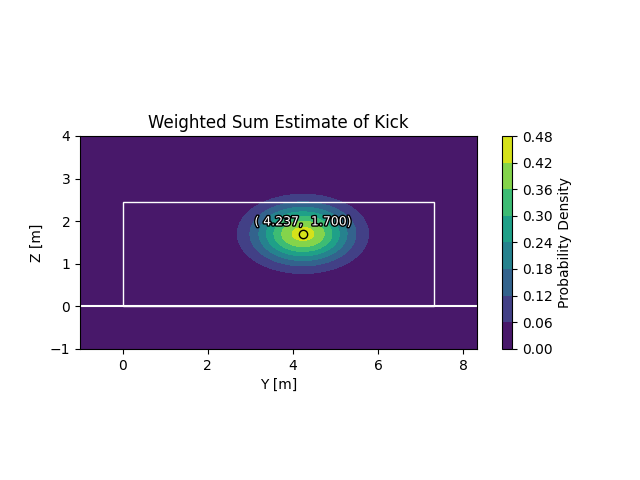
\includegraphics[width=0.99\textwidth]{Problem 2/out/weighted_sum_probability_dist.png}
    \caption{Kick prediction results}
    \label{fig:p2-weighted-sum-results}
\end{figure}


\section{Problem 3 - Neural Network Estimation of Walking Gate Ground Force}
Problem 3 focuses on using a Neural Network to estimate the ground reaction forces produced by a person walking. The input data is an array of 50 different measurements on the person's body. The goal is to predict the ground reaction force produced by the person instead of needing expensive and particular equipment to determine those values. The output is a 4 value vector representing the forces in the Y and Z directions from each of the left and right feet.

\subsection{Neural Network Design}
A rather simple approach was taken to the neural network design. The hope was that the neural network training would decide what values were important to the prediction and ignore whatever of the 50 values was not very relivant. The neural network was designed with 2 hidden layers, each with 100 nodes. Each hidden node used a sigmoid activation function since this is a relatively shallow network. The output layer used a linear activation function to allow for the output to be a continuous value. The rough architecture of the neural network is shown in figure \ref{fig:p3-nn-architecture}.

\begin{figure}[H]
    \centering
    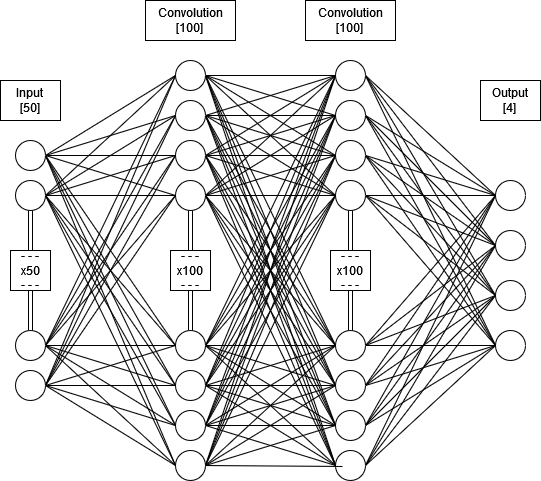
\includegraphics[width=0.75\textwidth]{Problem 3/assets/NeuralNet.png}
    \caption{Neural network architecture}
    \label{fig:p3-nn-architecture}
\end{figure}

\subsection{Neural Network Implementation}
The neural network was implemented in Python using TensorFlow \cite{tensorflow} and Keras \cite{keras}, specifically the Keras models computed in TensorFlow. The code for the neural network is shown in \ref{appendix-p3-code}.

\subsection{Neural Network Training}
The neural network was trained on subjects 1-8 of the provided data. Subject 9 was used as a validation set to ensure the neural network was not overfitting. Training was done in batches of 50 to vastly improve the speed of training. The neural network was trained for 100 epochs, with the possibility of breaking training early if there was a stagnation in the reduction of the root mean squared error. After each epoch, the model was tested against the validation set using the metrics of root mean squared error (RMSE) and the coefficient of determination ($\text{R}^2$). The training history is shown in figure \ref{fig:p3-training-history}.

\begin{figure}[H]
    \begin{subfigure}[b]{0.49\textwidth}
        \centering
        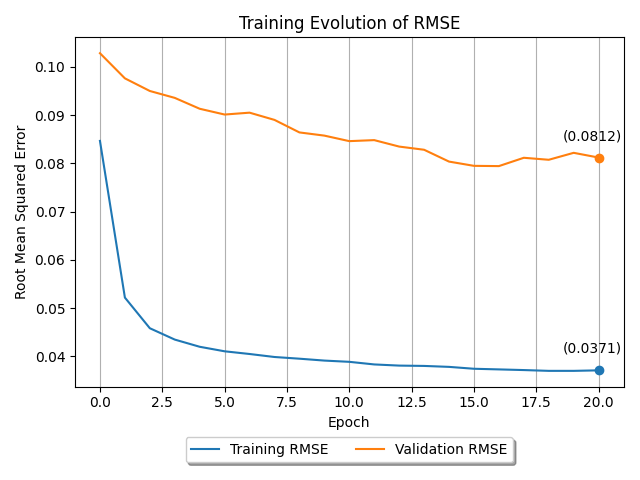
\includegraphics[width=\textwidth]{Problem 3/out/training_history_rmse.png}
        \caption{Root mean square error (RMSE)}
        \label{fig:p3-rmse-training-history}
    \end{subfigure}
    \begin{subfigure}[b]{0.49\textwidth}
        \centering
        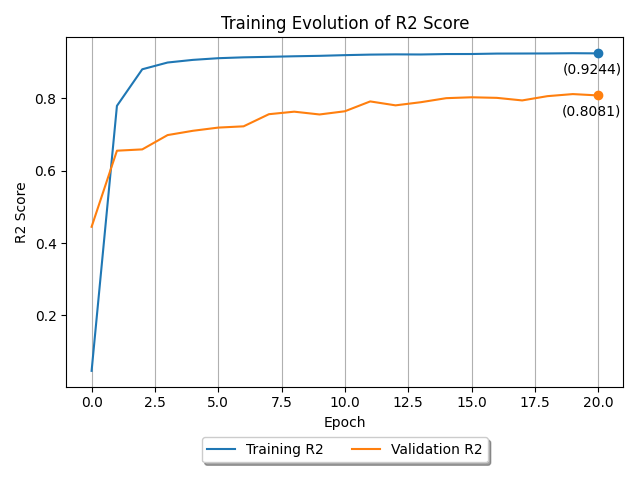
\includegraphics[width=\textwidth]{Problem 3/out/training_history_r2.png}
        \caption{$\text{R}^2$}
        \label{fig:p3-r2-training-history}
    \end{subfigure}
    \caption{Training history}
    \label{fig:p3-training-history}
\end{figure}

As to be expected, the improvement is rapid in the early epochs and slows toward the en. Due to the stagnation in the change of RMSE, the training was stopped at epoch 20. The final RMSE and $\text{R}^2$ values are shown in table \ref{tab:p3-training-results}.

\begin{table}[H]
    \centering
    \caption{Training results}
    \label{tab:p3-training-results}
    \begin{tabular}{|c|c|c|}
        \hline
        \textbf{Metric} & \textbf{Training Set} & \textbf{Validation Set}\\
        \hline
        RMSE & 0.0371 & 0.0812 \\
        \hline
        $\text{R}^2$ & 0.9244 & 0.8081\\
        \hline
    \end{tabular}
\end{table}

The training shows a significant improvement in the $\text{R}^2$ over the course of the 20 epochs. The RMSE is also quite low, showing that the neural network is able to predict the ground reaction forces with a high degree of accuracy.

\subsection{Neural Network Results}
The neural network was then used to predict the ground reaction forces of subject 10 for all 2000 measurements. As requested, a CSV file was prepared with the output of the neural network. The results are plotted in figure \ref{fig:p3-gate-rx-frc-est} in \ref{sec:appendix-gate-rx-frc-est}. The results show a reasonable estimation of the forces produced by the subject. The gate appears consistent and force scale between the left and right feet is also consistent.

% BIBLIOGRAPHY ──────────────────────────────────────────────────────────────────── %
\clearpage
\bibliographystyle{plain} % We choose the "plain" reference style
\bibliography{references} % Entries are in the references.bib file

% APPENDIX ──────────────────────────────────────────────────────────────────────── %
\clearpage
\section*{Appendices} \label{sec:appendix}
\addcontentsline{toc}{section}{\nameref{sec:appendix}}
\renewcommand\thesubsection{Appendix \Alph{subsection}}
\renewcommand\thesubsubsection{Appendix \Alph{subsection}-\arabic{subsubsection}}

\subsection{Gate Reaction Force Estimation} \label{sec:appendix-gate-rx-frc-est}
\begin{figure}[H]
    \centering
    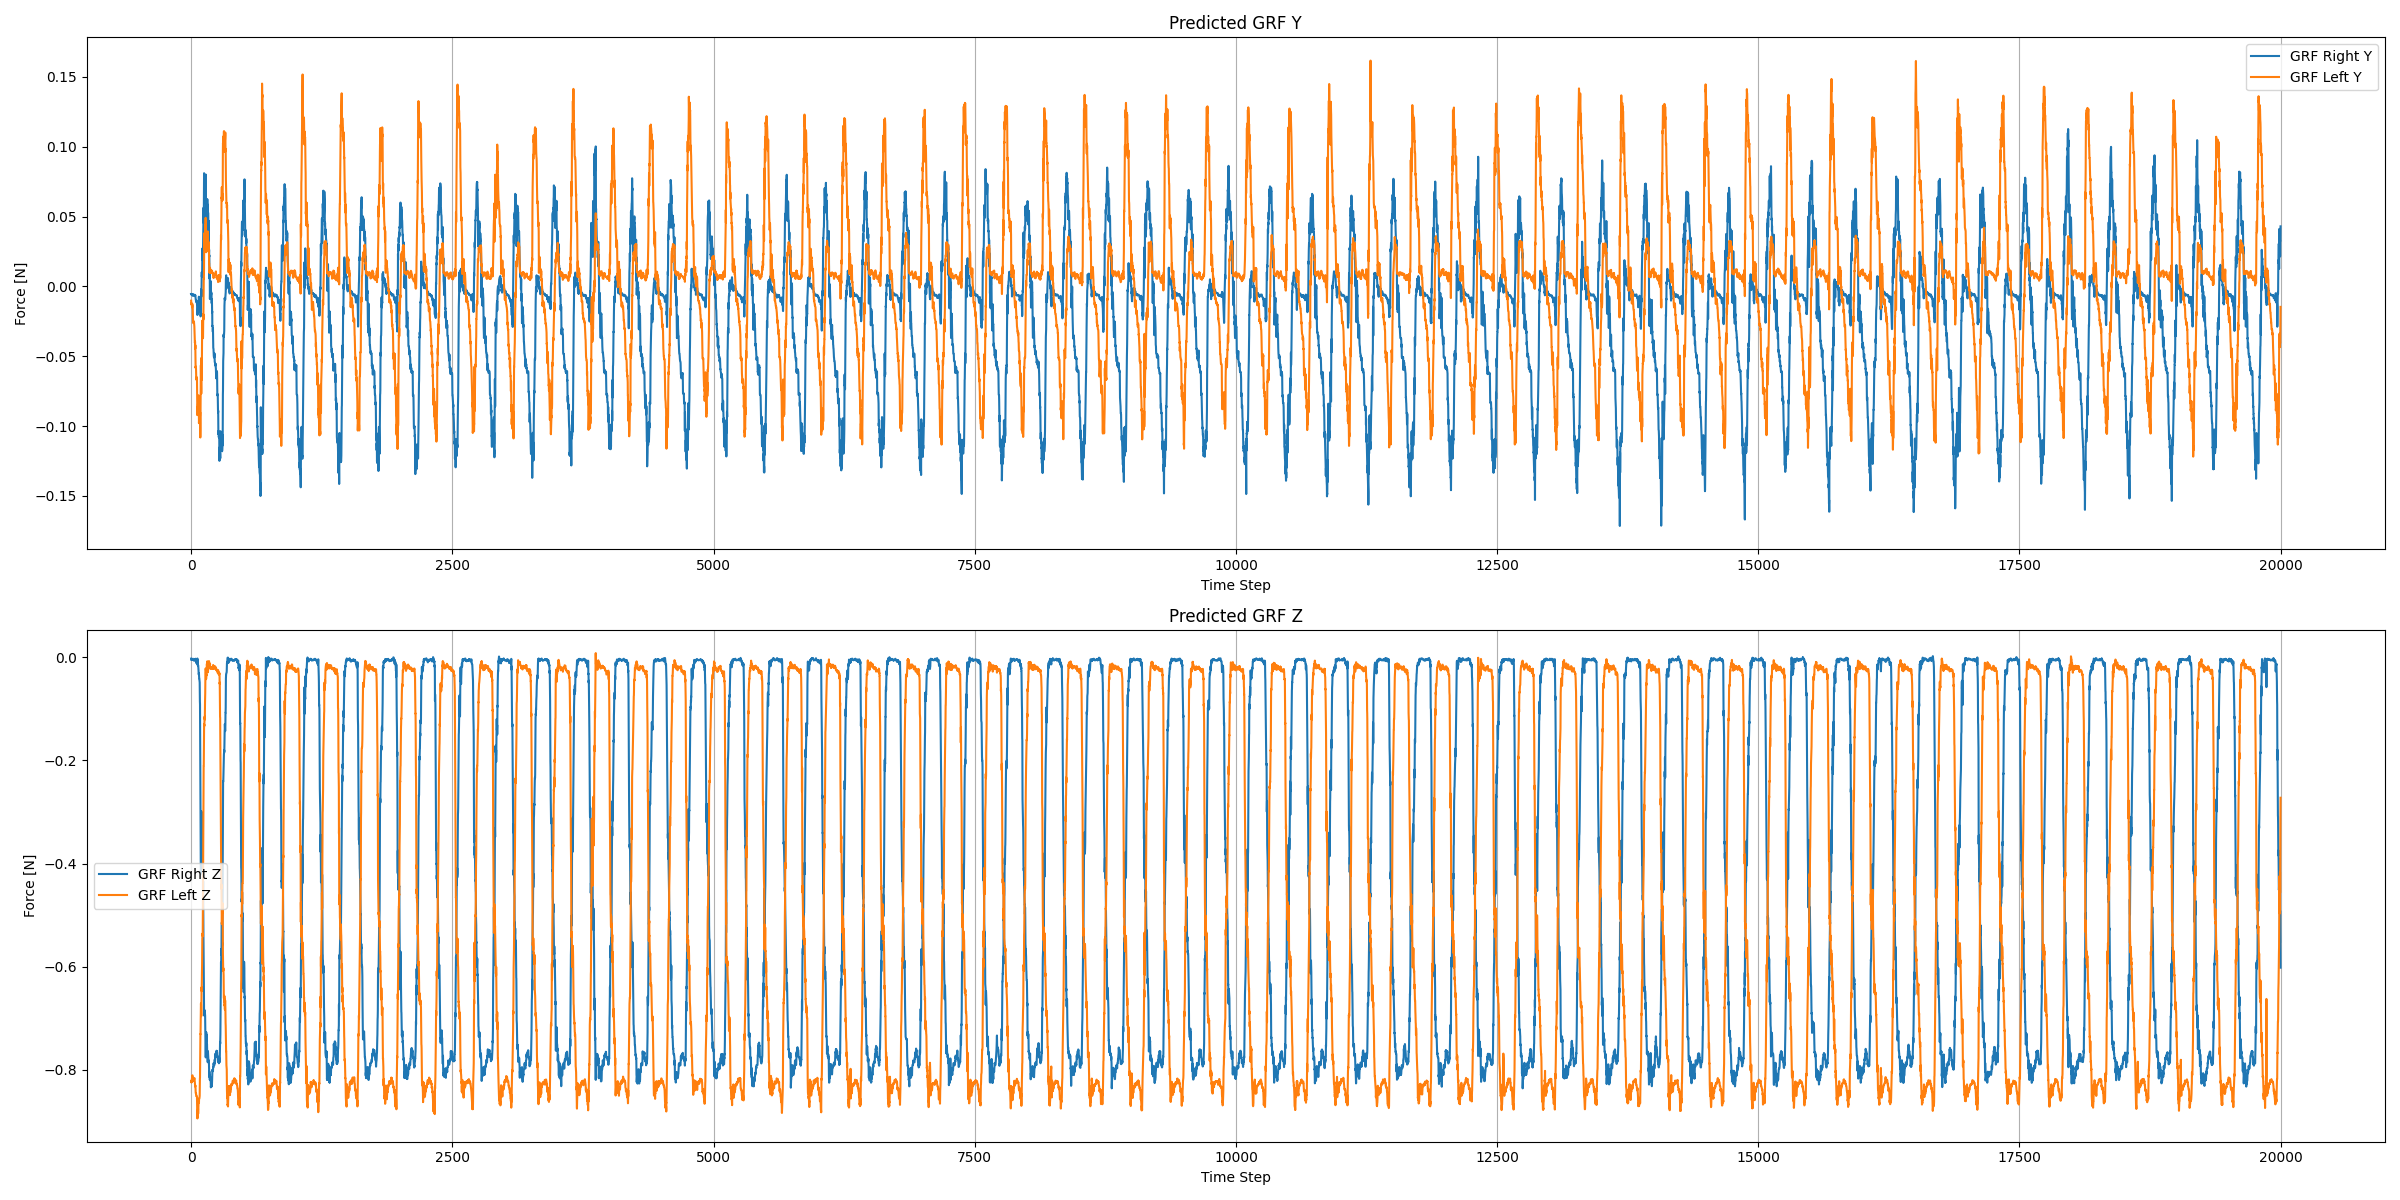
\includegraphics[angle=90, width=0.6\textwidth]{Problem 3/out/predictions.png}
    \caption{Gate reaction force estimation}
    \label{fig:p3-gate-rx-frc-est}
\end{figure}

\clearpage
\subsection{Problem 1 Source Code} \label{appendix-p1-code}
\lstinputlisting[language=Python]{Problem 1/out/Problem_1.py}
\clearpage
\subsection{Problem 2 Source Code} \label{appendix-p2-code}
\lstinputlisting[language=Python]{Problem 2/out/Problem_2.py}
\clearpage
\subsection{Problem 3 Source Code} \label{appendix-p3-code}
\lstinputlisting[language=Python]{Problem 3/out/Problem_3.py}

\end{document}
